% !Mode:: "TeX:UTF-8"

\def\xuewei{Doctor} % 定义学位 Doctor or Master
\documentclass[cs4size,openany,oneside,UTF8,nofonts]{ctexbook}
\usepackage[a4paper,text={160true mm,234true mm},top=30.5true mm,left=25true mm,head=5true mm,headsep=2.5true mm,foot=8.5true mm]{geometry}
\usepackage{ccaption}
\usepackage{booktabs}
\usepackage{longtable}
\usepackage{caption}
\usepackage{amsmath}
\usepackage{amssymb}
\usepackage{mathtools}
\usepackage{bigints}
\usepackage{bm}
\usepackage{txfonts}
\usepackage{graphicx}
\usepackage{enumitem}
\usepackage{fancyhdr}
\usepackage{ntheorem}
\usepackage{titlesec}
\usepackage{titletoc}                   % 控制目录的宏包
\usepackage{subfigure}
\usepackage{tabularx}
\usepackage[sort&compress,numbers]{natbib}
\usepackage[boxed,linesnumbered,algochapter]{algorithm2e}	
\usepackage{listings}
\lstset{ columns=flexible, breaklines=true }

\usepackage[xetex,
            bookmarksnumbered=true,
            bookmarksopen=true,
            colorlinks=false,
            pdfborder={0 0 1},
            citecolor=blue,
            linkcolor=red,
            anchorcolor=green,
            urlcolor=blue,
            breaklinks=true,
            naturalnames  %与algorithm2e宏包协调
            ]{hyperref}
%\usepackage[BoldFont,normalindentfirst,BoldFont,SlantFont]{xeCJK}
\defaultfontfeatures{Mapping=tex-text}
\xeCJKsetemboldenfactor{1}%只对随后定义的CJK字体有效
\setCJKfamilyfont{hei}{SimHei}
\xeCJKsetemboldenfactor{4}
\setCJKfamilyfont{song}{SimSun}
\xeCJKsetemboldenfactor{1}
\setCJKfamilyfont{fs}{FangSong}
\setCJKfamilyfont{kai}{KaiTi}
\setCJKfamilyfont{li}{LiSu}
\setCJKfamilyfont{xw}{STXinwei}
\setCJKmainfont{SimSun}
\setCJKsansfont{SimHei}
\setmainfont{Times New Roman}
\setsansfont{Arial}
\newcommand{\heiti}{\CJKfamily{hei}}% 黑体   (Windows自带simhei.ttf)
\newcommand{\songti}{\CJKfamily{song}}    % 宋体   (Windows自带simsun.ttf)
\newcommand{\fs}{\CJKfamily{fs}}        % 仿宋体 (Windows自带simfs.ttf)
\newcommand{\kaishu}{\CJKfamily{kai}}      % 楷体   (Windows自带simkai.ttf)
\newcommand{\li}{\CJKfamily{li}}        % 隶书   (Windows自带simli.ttf)
\newcommand{\xw}{\CJKfamily{xw}}        % 隶书   (Windows自带simli.ttf)
\newfontfamily\arial{Arial}
\newfontfamily\timesnewroman{Times New Roman}


\newcommand{\yihao}{\fontsize{26pt}{26pt}\selectfont}       % 一号, 1.倍行距
\newcommand{\xiaoyi}{\fontsize{24pt}{24pt}\selectfont}      % 小一, 1.倍行距
\newcommand{\erhao}{\fontsize{22pt}{1.25\baselineskip}\selectfont}       % 二号, 1.倍行距
\newcommand{\xiaoer}{\fontsize{18pt}{18pt}\selectfont}      % 小二, 单倍行距
\newcommand{\sanhao}{\fontsize{16pt}{16pt}\selectfont}      % 三号, 1.倍行距
\newcommand{\xiaosan}{\fontsize{15pt}{15pt}\selectfont}     % 小三, 1.倍行距
\newcommand{\sihao}{\fontsize{14pt}{14pt}\selectfont}       % 四号, 1.0倍行距
\newcommand{\xiaosi}{\fontsize{12pt}{12pt}\selectfont}      % 小四, 1.倍行距
\newcommand{\wuhao}{\fontsize{10.5pt}{10.5pt}\selectfont}   % 五号, 单倍行距
\newcommand{\xiaowu}{\fontsize{9pt}{9pt}\selectfont}        % 小五, 单倍行距

\newcommand\litem[1]{\item{\heiti#1\hspace{1.5em}}}

\newenvironment{listitem}{\begin{enumerate}[label={(\arabic*)},itemindent=2em]}{\end{enumerate}}

\usepackage[boxed,linesnumbered,algochapter]{algorithm2e}  % 算法的宏包,注意宏包兼容性,先后顺序为float、hyperref、algorithm(2e),否则无法生成算法列表
\renewcommand{\algorithmcfname}{算法}

\usepackage{tikz,mathpazo}

\usetikzlibrary{shapes.geometric, arrows}

\newcommand{\citeayu}[1]{\citeauthor{#1}~(\citeyear{#1})\citeup{#1}}

\begin{document}

\titleformat{\chapter}{\center\xiaoer\hei}{\chaptertitlename}{0em}{}
\titlespacing{\chapter}{0pt}{0.5\bseieskip}{0.5\bseieskip}
\titleformat{\section}{\xiaosan\hei}{\thesection}{0em}{}
\titlespacing{\section}{0pt}{0.5\bseieskip}{0.5\bseieskip}
\titleformat{\subsection}{\sihao\hei}{\thesubsection}{0em}{}
\titlespacing{\subsection}{0pt}{0.5\bseieskip}{0.5\bseieskip}
\titleformat{\subsubsection}{\xiaosi\hei}{\thesubsubsection}{0em}{}
\titlespacing{\subsubsection}{0pt}{0pt}{0pt}

\newif\ifxueweidoctor
\newif\ifxueweimaster
\def\temp{Doctor}
\ifx\temp\xuewei
  \xueweidoctortrue  \xueweimasterfalse
\fi
\def\temp{Master}
\ifx\temp\xuewei
  \xueweidoctorfalse  \xueweimastertrue
\fi

% !Mode:: "TeX:UTF-8" 
\setlength{\subfigbottomskip}{0pt}
\CTEXoptions[bibname={主要参考文献}]
\CTEXsetup[name={,},number={}]{chapter}
\captionsetup{labelsep=space,font=small,justification=centering}
\arraycolsep=1.7pt
\graphicspath{{figures/}}
\renewcommand{\subcapsize}{\zihao{5}}
\renewcommand{\thesubfigure}{\alph{subfigure})}
\setcounter{secnumdepth}{4}
\newcommand{\pozhehao}{\raisebox{0.1em}{------}}
\titleformat{\chapter}{\center\zihao{-2}\heiti}{\chaptertitlename}{0.5em}{}
\titlespacing{\chapter}{0pt}{-4.5mm}{8mm}
\titleformat{\section}{\zihao{-3}\heiti}{\thesection}{0.5em}{}
\titlespacing{\section}{0pt}{4.5mm}{4.5mm}
\titleformat{\subsection}{\zihao{4}\heiti}{\thesubsection}{0.5em}{}
\titlespacing{\subsection}{0pt}{4mm}{4mm}
\titleformat{\subsubsection}{\zihao{-4}\heiti}{\thesubsubsection}{0.5em}{}
\titlespacing{\subsubsection}{0pt}{0pt}{0pt}
\makeatletter
\renewcommand\thesection{\@arabic \c@section} % 前面不带 thechapter
\makeatother

\theoremstyle{plain}
\theorembodyfont{\songti\rmfamily}
\theoremheaderfont{\heiti\rmfamily}
\newtheorem{definition}{\heiti 定义}
\newtheorem{example}{\heiti 例}
\newtheorem{algo}{\heiti 算法}
\newtheorem{theorem}{\heiti 定理}
\newtheorem{axiom}{\heiti 公理}
\newtheorem{proposition}{\heiti 命题}
\newtheorem{lemma}{\heiti 引理}
\newtheorem{corollary}{\heiti 推论}
\newtheorem{remark}{\heiti 注解}
\newenvironment{proof}{\noindent{\heiti 证明:}}{\hfill $ \square $ \vskip 4mm}
\theoremsymbol{$\square$}

% 定义页眉和页脚 使用fancyhdr 宏包
\newcommand{\makeheadrule}{
\rule[7pt]{\textwidth}{0.75pt} \\[-23pt]
\rule{\textwidth}{2.25pt}}
\renewcommand{\headrule}{
    {\if@fancyplain\let\headrulewidth\plainheadrulewidth\fi
     \makeheadrule}}
\makeatother
		
\pagestyle{fancyplain}
\renewcommand{\chaptermark}[1]{\relax}
\renewcommand{\sectionmark}[1]{\markright{#1}}
\fancyhf{}
\ifxueweidoctor
  \fancyhead[CO]{\songti \zihao{-5}\rightmark}
  \fancyhead[CE]{\songti \zihao{-5} 哈尔滨工业大学博士学位论文开题报告}%
  \fancyfoot[C]{\zihao{-5} -~\thepage~-}
	\renewcommand\bibsection{\section*{\centerline{\bibname}}
	\markboth{哈尔滨工业大学博士学位论文开题报告}{\bibname}}
\fi
\ifxueweimaster
  \fancyhead[C]{\songti \zihao{-5} 哈尔滨工业大学硕士学位论文开题报告}
  \fancyfoot[C]{\zihao{-5} -~\thepage~-}
	\renewcommand\bibsection{\section*{\centerline{\bibname}}
	\markboth{哈尔滨工业大学硕士学位论文开题报告}{\bibname}}
\fi

\renewcommand{\CJKglue}{\hskip 0.56pt plus 0.08\baselineskip} %加大字间距,使每行33个字
\def\defaultfont{\renewcommand{\baselinestretch}{1.62}\normalsize\selectfont}
% 调整罗列环境的布局
\setitemize{leftmargin=3em,itemsep=0em,partopsep=0em,parsep=0em,topsep=-0em}
\setenumerate{leftmargin=3em,itemsep=0em,partopsep=0em,parsep=0em,topsep=0em}
\renewcommand{\theequation}{\arabic{equation}}
\renewcommand{\thetable}{\arabic{table}}
\renewcommand{\thefigure}{\arabic{figure}}

\makeatletter
\renewcommand{\p@subfigure}{\thefigure~}
\makeatother

\newcommand{\citeup}[1]{\textsuperscript{\cite{#1}}} % for WinEdt users

% 封面、摘要、版权、致谢格式定义
\makeatletter
\def\title#1{\def\@title{#1}}\def\@title{}
\def\titlesec#1{\def\@titlesec{& \rule[-4pt]{200pt}{1pt}\hspace{-326pt}\centerline{\textbf{#1}}}}\def\@titlesec{}
\def\affil#1{\def\@affil{#1}}\def\@affil{}
\def\subject#1{\def\@subject{#1}}\def\@subject{}
\def\author#1{\def\@author{#1}}\def\@author{}
\def\bdate#1{\def\@bdate{#1}}\def\@bdate{}
\def\supervisor#1{\def\@supervisor{#1}}\def\@supervisor{}
\def\assosupervisor#1{\def\@assosupervisor{\textbf{副\hfill 导\hfill 师} & \rule[-4pt]{200pt}{1pt}\hspace{-326pt}\centerline{\textbf {#1}}\\}}\def\@assosupervisor{}
\def\cosupervisor#1{\def\@cosupervisor{\textbf{联\hfill 合\hfill 导\hfill 师} & \rule[-4pt]{200pt}{1pt}\hspace{-326pt}\centerline{\textbf {#1}}\\}}\def\@cosupervisor{}
\def\date#1{\def\@date{#1}}\def\@date{}
\def\stuno#1{\def\@stuno{#1}}\def\@stuno{}
% 定义封面
\ifxueweidoctor
\def\makecover{
    \thispagestyle{empty}
    \zihao{-2}\vspace*{10mm}
		\renewcommand{\CJKglue}{\hskip 2pt plus 0.08\baselineskip}
    \centerline{\heiti\textbf{哈尔滨工业大学}}
		\vspace{10mm}
		\centerline{\zihao{2}\songti\textbf{博士学位论文开题报告}}
    \zihao{-2}\vspace*{10mm}
		\renewcommand{\CJKglue}{\hskip 2pt plus 0.08\baselineskip}
    \centerline{\songti\textbf{题目:\textbf\@title}}
		\renewcommand{\CJKglue}{\hskip 0pt plus 0.08\baselineskip}
    \zihao{3}\vspace{4\baselineskip}
    \hspace*{36pt}{\songti
	\renewcommand{\arraystretch}{1.3}
    \begin{tabular}{l@{}l}
    \textbf{院\hfill (系)}   & \rule[-4pt]{200pt}{1pt}\hspace{-326pt}\centerline{\textbf\@affil}\\
    \textbf{学\hfill 科}     & \rule[-4pt]{200pt}{1pt}\hspace{-326pt}\centerline{\textbf\@subject}\\
    \textbf{导\hfill 师}     & \rule[-4pt]{200pt}{1pt}\hspace{-326pt}\centerline{\textbf\@supervisor}\\
    \textbf{研\hfill 究\hfill 生}      & \rule[-4pt]{200pt}{1pt}\hspace{-326pt}\centerline{\textbf\@author}\\
    \textbf{学\hfill 号}  & \rule[-4pt]{200pt}{1pt}\hspace{-326pt}\centerline{\textbf\@stuno}\\
    \textbf{开题报告日期} & \rule[-4pt]{200pt}{1pt}\hspace{-326pt}\centerline{\textbf\@date}\\
    \end{tabular}\renewcommand{\arraystretch}{1}}
	\vfill
    \centerline{\songti\textbf{研究生院制}}
    \vspace{0.5\baselineskip}
    \centerline{\songti\textbf{二〇一四年九月}}

%%定义内封
    %%新版本没有内封
%\newpage
%\thispagestyle{empty}
%\zihao{5}\vspace*{2em}
%\begin{center}
%  \heiti\zihao{3}说\hspace{3em}明
%\end{center}
%\vspace*{40pt}
%	\renewcommand{\arraystretch}{1.25}
%    {\songti\zihao{5}
%    \hangindent=2em\noindent 一、开题报告应包括下列主要内容:
%    \begin{enumerate}[leftmargin=36pt]
%    \item 课题来源及研究的目的和意义;
%    \item 国内外在该方向的研究现状及分析(文献综述);
%    \item 前期的理论研究与试验论证工作的结果;
%    \item 学位论文的主要研究内容、实施方案及其可行性论证;
%    \item 论文进度安排,预期达到的目标;
%    \item 为完成课题已具备和所需的条件、外协计划及经费;
%    \item 预计研究过程中可能遇到的困难、问题,以及解决的途径;
%    \item 主要参考文献(应在~50~篇以上,其中外文资料不少于二分之一,参考文献中近五年内发表的文献一般不少于三分之一,且必须有近二年内发表的文献资料)。
%    \end{enumerate}
%    \noindent 二、开题报告字数应不少于~1.5~万字。
%
%    \noindent 三、开题报告时间应最迟应于第四学期结束前完成。
%
%    \hangindent=2em\noindent 四、若本次开题报告未通过,需在三个月内再次进行开题报告。第二次学位论文开题报告
%    仍未通过者,将取消其学籍。
%
%    \hangindent=2em\noindent 五、开题报告结束后,评议小组要填写《博士学位论文开题报告评议结果》上报院(系)研
%    究生教学秘书备案。
%
%    \noindent 六、此表不够填写时,可另加附页。
%    }
%	\renewcommand{\arraystretch}{1}
    \clearpage
}
\fi

\ifxueweimaster
\def\makecover{
    \thispagestyle{empty}
    \zihao{-2}\vspace*{10mm}
		\renewcommand{\CJKglue}{\hskip 2pt plus 0.08\baselineskip}
    \centerline{\kaishu\textbf{哈尔滨工业大学}}
		
		\vspace{10mm}
		\centerline{\zihao{2}\songti\textbf{硕士学位论文开题报告}}

		\renewcommand{\CJKglue}{\hskip 0pt plus 0.08\baselineskip}
\vspace{30pt}
\zihao{-2}
\begin{center}\songti\textbf{题~目:\@title}\end{center}
\vspace{30pt}
    \zihao{3}
    \hspace*{68pt}{\songti
	\renewcommand{\arraystretch}{1.3}
    \begin{tabular}{l@{}l}
    \textbf{院\hfill (系)}   & \rule[-4pt]{200pt}{1pt}\hspace{-326pt}\centerline{\textbf\@affil}\\
    \textbf{学\hfill 科}     & \rule[-4pt]{200pt}{1pt}\hspace{-326pt}\centerline{\textbf\@subject}\\
    \textbf{导\hfill 师}     & \rule[-4pt]{200pt}{1pt}\hspace{-326pt}\centerline{\textbf\@supervisor}\\
    \@assosupervisor
	\@cosupervisor
    \textbf{研\hfill 究\hfill 生}      & \rule[-4pt]{200pt}{1pt}\hspace{-326pt}\centerline{\textbf\@author}\\
    \textbf{学\hfill 号}  & \rule[-4pt]{200pt}{1pt}\hspace{-326pt}\centerline{\textbf\@stuno}\\
    \textbf{开题报告日期} & \rule[-4pt]{200pt}{1pt}\hspace{-326pt}\centerline{\textbf\@date}\\
    \end{tabular}
		\renewcommand{\arraystretch}{1}}
	\vfill
    \centerline{\songti\textbf{研究生院培养处制}}

%%定义内封
\newpage
\thispagestyle{empty}
\zihao{5}\vspace*{2em}
\begin{center}
  \heiti\zihao{3}说\hspace{3em}明
\end{center}
\vspace*{40pt}
	\renewcommand{\arraystretch}{1.25}
    {\songti\zihao{5}
    \hangindent=2em
	\noindent 一、开题报告应包括下列主要内容:
    \begin{enumerate}[leftmargin=36pt]
	\item 课题来源及研究的目的和意义;
	\item 国内外在该方向的研究现状及分析;
	\item 主要研究内容;
	\item 研究方案及进度安排,预期达到的目标;
	\item 为完成课题已具备和所需的条件和经费;
	\item 预计研究过程中可能遇到的困难和问题,以及解决的措施;
	\item 主要参考文献。
    \end{enumerate}
    \noindent 二、对开题报告的要求
	\begin{enumerate}[leftmargin=36pt]
	\item 开题报告的字数应在~5000~字以上;
	\item 阅读的主要参考文献应在~20~篇以上,其中外文资料应不少于三分之一。硕士研究生应在导师的指导下着重查阅近年内发表的中、\hspace{-1pt}外文期刊文章。\hspace{-1pt}本学科的基础和专业课教材一般不应列为参考资料。
    \end{enumerate}
    \noindent 三、开题报告时间应最迟不得超过第三学期的第三周末。

    \hangindent=2em\noindent 四、如硕士生首次开题报告未通过,\hspace{-2pt}需在一个月内再进行一次。\hspace{-3pt}若仍不通过,\hspace{-2pt}则停止硕士论文工作。

    \noindent 五、此表不够填写时,可另加附页。

\hangindent=2em\noindent 六、开题报告进行后,此表同硕士学位论文开题报告评议结果存各系(院)研究生秘书书处,以备研究生院及所属学院进行检查。

    }
	\renewcommand{\arraystretch}{1}
    \clearpage
}
\fi
\makeatother

% !Mode:: "TeX:UTF-8"

\affil{机电工程学院}
\subject{机械制造及其自动化}
\author{于冬梅}
\supervisor{某某某教授}
\assosupervisor{副导名}%若无副导师,请屏蔽掉此句
\cosupervisor{联导名}%若无联合导师,请屏蔽掉此句
\date{2011年7月20日}
\stuno{09S906001}
\bdate{2009年9月}

\ifxueweidoctor
  \title{局部多孔质气体静压轴承} %论文题目,此处最多12个字,题目剩余的字放在\ctitlesec里面
  \titlesec{关键技术的研究}
\fi
\ifxueweimaster
  \title{局部多孔质气体静压轴承关键技术的研究}
\fi

\makecover
\clearpage
\setcounter{page}{1} 
\zihao{-4}
\tableofcontents    % 中文目录
\chapter*{局部多孔质气体静压轴承关键技术的研究}
% !Mode:: "TeX:UTF-8" 
\section{图片的插入方法}
\subsection{研究生院的插图规范}
图应有自明性。插图应与文字紧密配合,文图相符,内容正确。选图要力求精练,插图、照片应完整清晰。图中文字和数字等字号用宋体~5~号字。

机械工程图:采用第一角投影法,严格按照~GB4457~GB131-83《机械制图》标准规定。

数据流程图、程序流程图、系统流程图等按~GB1526-89~标准规定。

电气图:图形符号、文字符号等应符合附录~3~所列有关标准的规定。

流程图:必须采用结构化程序并正确运用流程框图。

对无规定符号的图形应采用该行业的常用画法。

坐标图的坐标线均用细实线,粗细不得超过图中曲线,有数字标注的坐标图,必须注明坐标单位。

照片图要求主题和主要显示部分的轮廓鲜明,便于制版。如用放大或缩小的复制品,必须清晰,反差适中。照片上应有表示目的物尺寸的标度。

引用文献图表必须标注出处。


\subsubsection{图题及图中说明}
每个图均应有图题(由图序和图名组成),图名在图序之后空一格排写。图序按章编排,如第~1~章第一个插图的图号为“图~1-1”等。
图题置于图下,硕士论文可只用中文书写,博士论文用中、英文两种文字居中书写,中文在上,要求中文用宋体~5~号字,英文用~Times New Roman 5~号字。有图注或其它说明时应置于图题之上。引用图应注明出处,在图题右上角加引用文献号。
图中若有分图时,分图题置于分图之下或图题之下,分图号用~a)、b)等表示。

图中各部分说明应采用中文(引用的外文图除外)或数字项号,各项文字说明置于图题之上(有分图题者,置于分图题之上)。

\subsubsection{插图编排}
插图之前,文中必须有关于本插图的提示,如“见图~1-1”、“如图~1-1~所示”等。插图与其图题为一个整体,不得拆开排写于两页。
插图处的该页空白不够排写该图整体时,则可将其后文字部分提前排写,将图移到次页。

\subsection{\LaTeX~中推荐使用的图片格式}
在~\LaTeX~中应用最多的图片格式是~EPS(Encapsulated PostScript)格式,它是一种专用的打印机描述语言,常用于印刷或打印输出。
EPS~格式图片可通过多种方式生成,这里介绍一款功能强大的免费图片处理软件------ImageMagick,
360~软件管家也提供此软件的下载。此软件可将其它格式图片转换为~EPS~格式图片,同时还可以锐化图片,使图片的局部清晰一些。

此软件对图片的格式转换操作都是在命令提示符(cmd.exe)中实现的,可以通过“开始$\to$运行$\to$输入~cmd$\to$回车”或
“开始$\to$程序$\to$附件$\to$命令提示符”找到它。在命令提示符下,首先采用“盘符命令”或“cd~命令”将当前目录改为待处理图片所在的目录,
在此目录下就可通过~convert~命令将图片转换为~EPS~格式,其命令的语法格式为

\noindent\verb|convert [可选参数] 原文件名.原扩展名 新文件名.eps|

\noindent 若~convert~命令中无可选参数,则将原来的图片格式直接转换为~EPS~格式,对图片不进行任何处理,这也是最常用的方法。
也可以选用可选参数,可选参数有很多选择,但最常用的有如下两个:

\verb|-sharpen radius{xsigma}|———此参数用来锐化图片,一般用在图片像素不高,需要提高图片清晰度的情况下。其中~radius~只能为整数,
它用来确定转换命令采取哪一种锐化算法,我们可以只取~radius~为~0;sigma~为所采取算法的锐化度,它的取值为~0.1--3~之间的任意一个浮点数,
数值越大,锐化程度也越大,通常取为~0.5--1~之间;x在参数中为分隔符。

\verb|-resize geometry|———此参数用来改变图片的大小,若图片的存储空间过大,可通过此命令缩小图片尺寸,但同时也将导致图片像素降低,
其具体用法请参见-resize geometry~的官方说明~http://www.imagemagick.org/script/command-line-options.php\#resize。

除此之外,一些文字处理软件和科学计算软件也支持生成~EPS~格式的文件,请使用“另存为”功能查看某款软件是否能够将图片以~EPS~格式的形式保存。

\subsection{单张图片的插入方法}
单张图片独自占一行的插入形式如图~\ref{golfer1}~所示。
\begin{figure}[htbp]
\centering
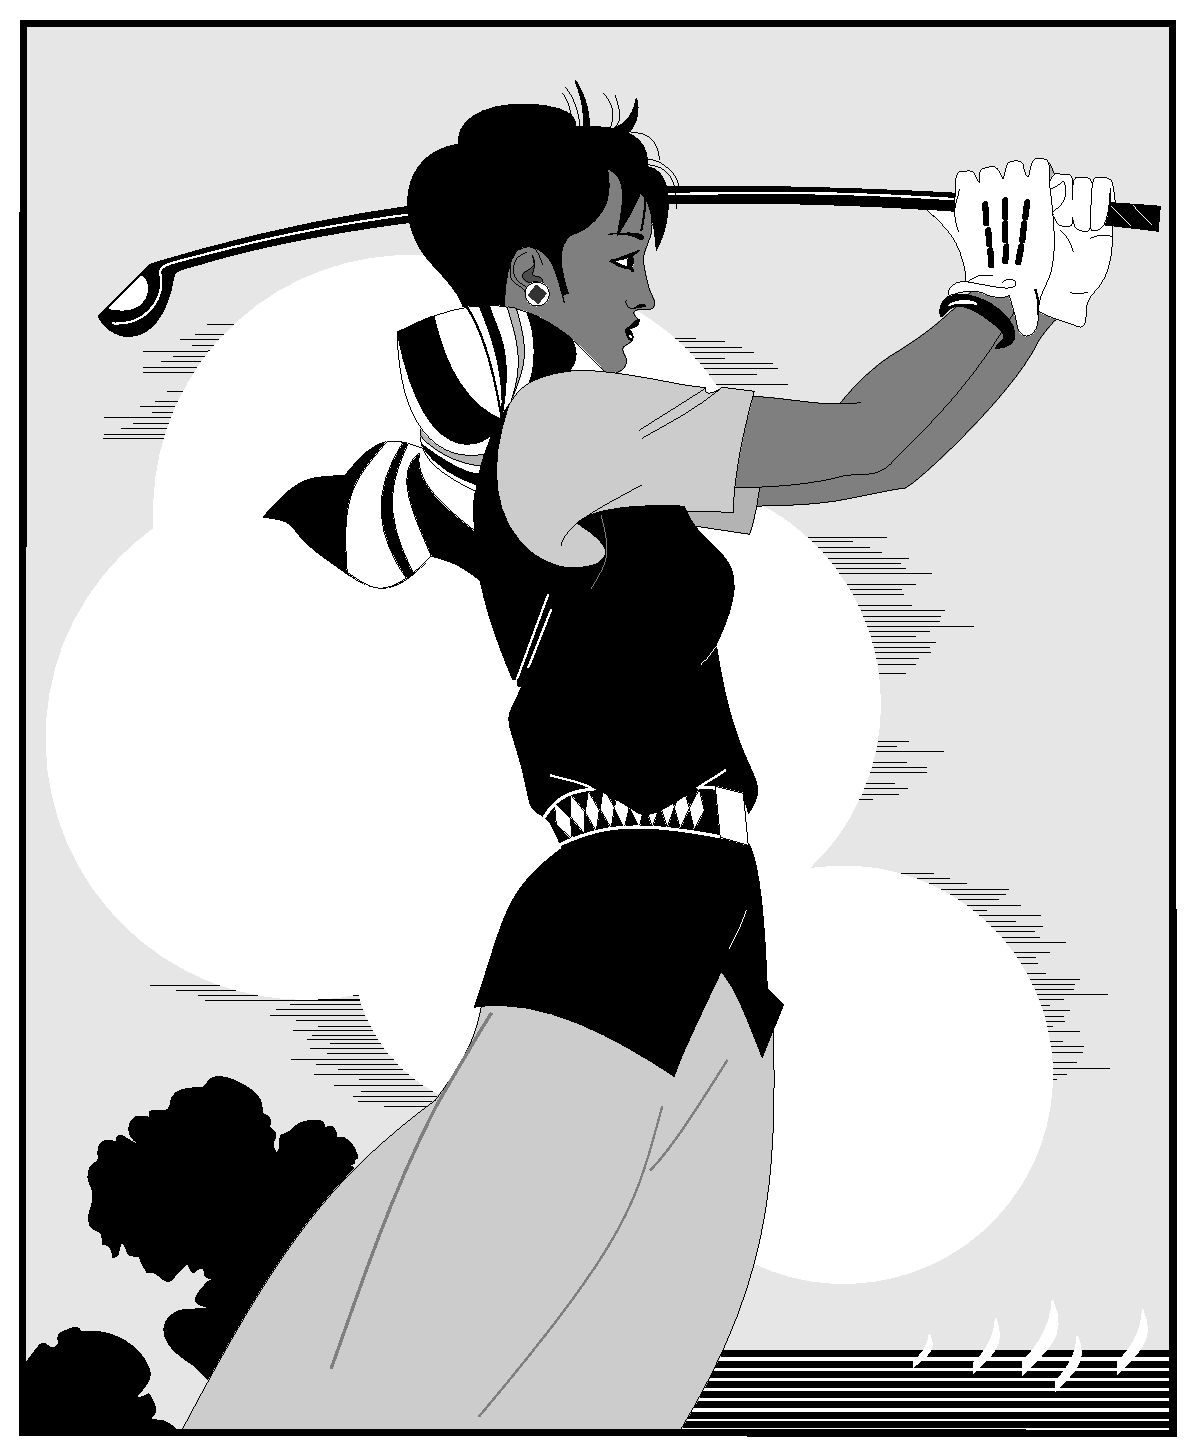
\includegraphics[width = 0.4\textwidth]{golfer}
\caption{打高尔夫球的人}\label{golfer1}
\vspace{-1em}
\end{figure}

其插入图片的代码及其说明如下。
\vspace{1em}\noindent\hrule
\begin{verbatim}
\begin{figure}[htbp]
\centering
\includegraphics[width=0.4\textwidth]{文件名(.eps)}
\caption{图片标题}\label{标签名(英文)}\vspace{-1em}
\end{figure}
\end{verbatim}
\noindent\hrule
\begin{verbatim}
figure环境的可选参数[htbp]表示浮动图形所放置的位置,h (here)表示当前位置,t (top)表示页芯顶部,b (bottom)表示页芯底部,p (page)表示单独一页。在word等软件中,图片通常插入到当前位置,如果当前页的剩余空间不够,图片将被移动到下一页,当前页就会出现很大的空白,其人工调整工作非常不便。由LaTeX提供的浮动图片功能,总是会按h->t->b->p的次序处理选项中的字母,自动调整图片的位置,大大减轻了工作量。
\centering命令将后续内容转换成每行皆居中的格式。
“\includegraphics”的可选参数用来设置图片插入文中的水平宽度,一般表示为正文宽度(\textwidth)的倍数。
\caption命令可以为图片或表格插入标题。
\label可为图片、表格或公式设置英文标签,一般不以图片或表格的数字顺序作为标签,而应包含一定的图片或表格信息,以便于文中引用(若图片、表格、公式、章节和参考文献等在文中出现的先后顺序发生了变化,其标注序号及其文中引用序号也会跟着发生变化,这一点是word等软件所不能做到的)。另外,图题或表题并不会因为分页而与图片或表格体分置于两页,章节等各级标题也不会置于某页的最底部,LaTeX系统会自动调整它们在正文中的位置,这也是word等软件所无法匹敌的。
\vspace将产生一定高度的竖直空白,必选参数为负值表示将后续文字位置向上提升,参数值可自行调整。em为长度单位,相当于大写字母M的宽度。
引用方法:“见图~\ref{标签名(英文)}”、“如图~\ref{标签名(英文)}~所示”等。
\end{verbatim}
\noindent\hrule\vspace{1em}
若需要将~2~张及以上的图片并排插入到一行中,则需要采用\verb|minipage|环境,如图~\ref{golfer2}~和图~\ref{golfer3}~所示。
\begin{figure}[htbp]
\centering
\begin{minipage}{0.4\textwidth}
\centering
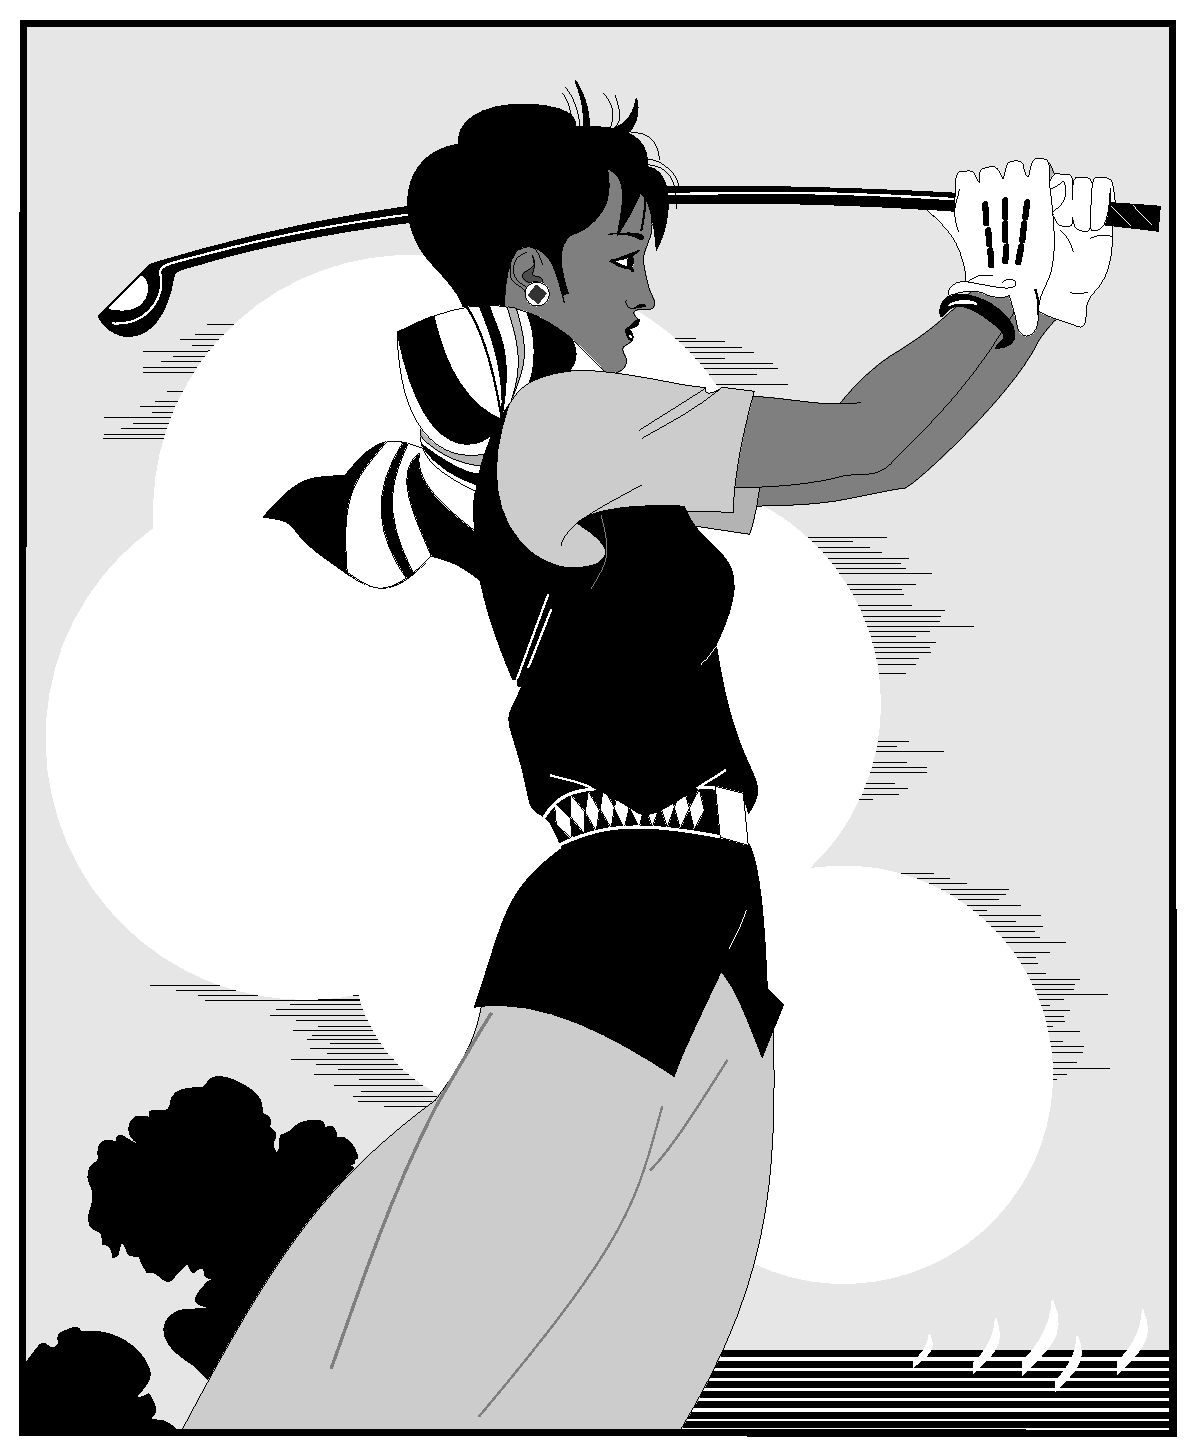
\includegraphics[width=\textwidth]{golfer}
\caption{打高尔夫球的人}\label{golfer2}
\end{minipage}
\begin{minipage}{0.4\textwidth}
\centering
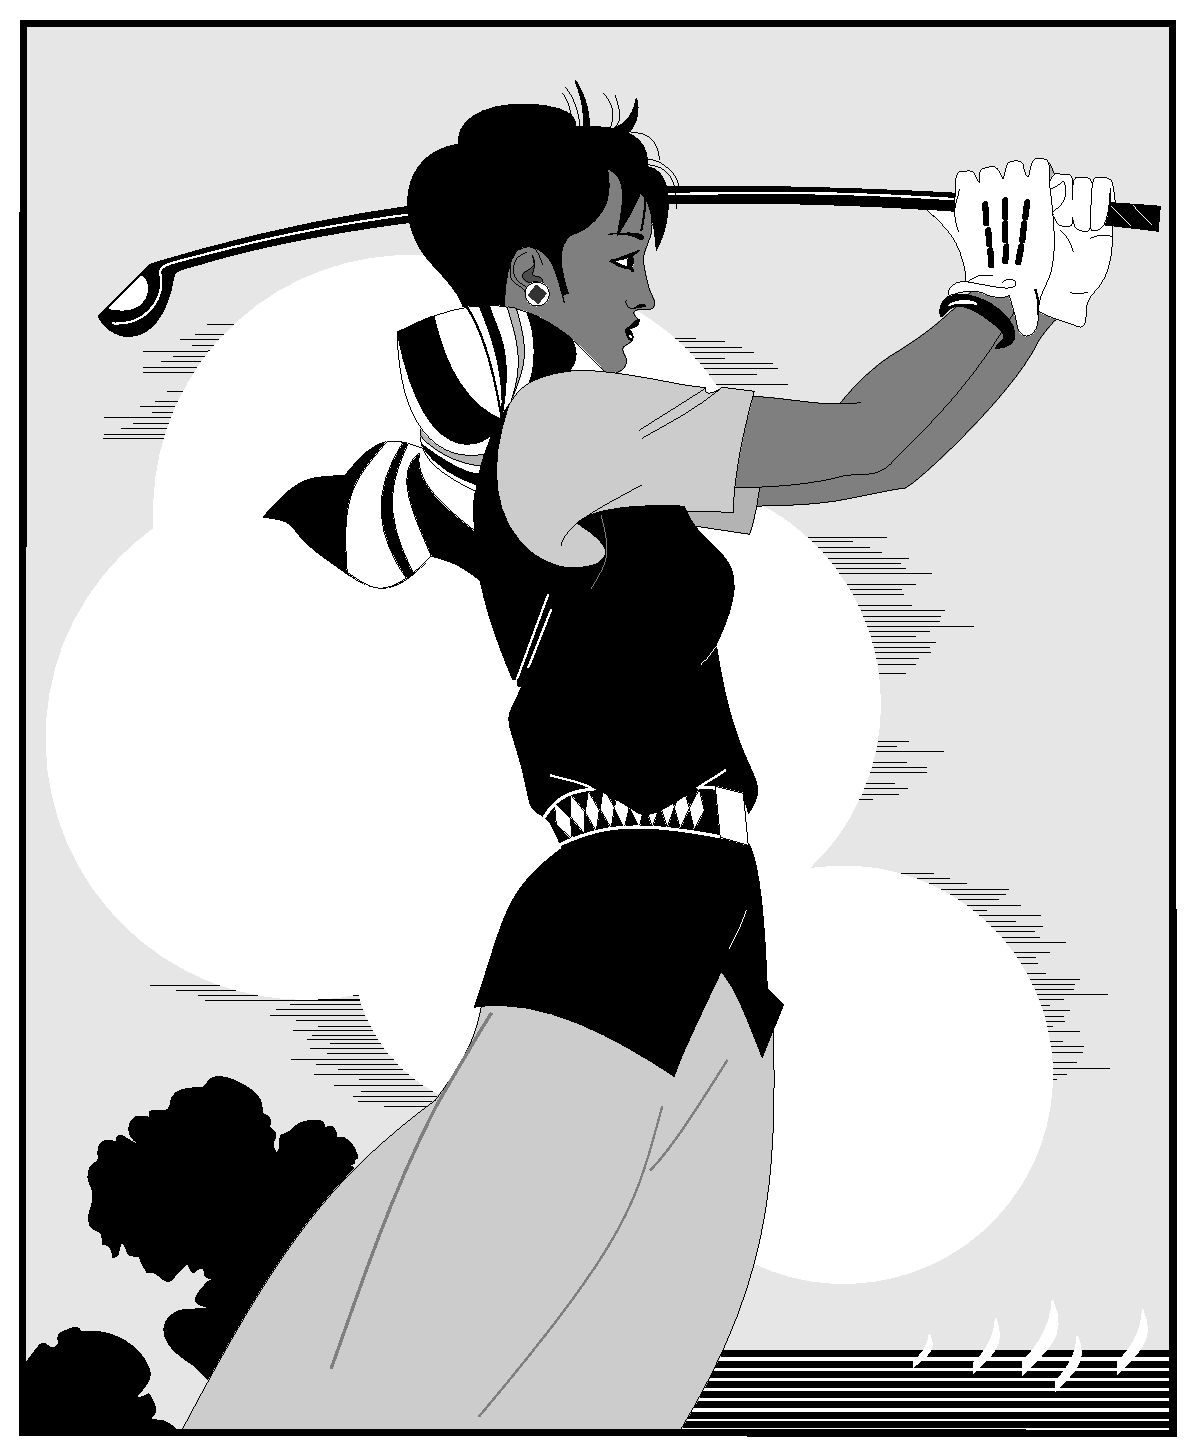
\includegraphics[width=\textwidth]{golfer}
\caption{打高尔夫球的人}\label{golfer3}
\end{minipage}\vspace{-1em}
\end{figure}

其代码如下所示。
\vspace{1em}\noindent\hrule
\begin{verbatim}
\begin{figure}[htbp]
\centering
\begin{minipage}{0.4\textwidth}
\centering
\includegraphics[width=\textwidth]{文件名}
\caption{图片标题}\label{标签名}
\end{minipage}
\begin{minipage}{0.4\textwidth}
\centering
\includegraphics[width=\textwidth]{文件名}
\caption{图片标题}\label{标签名}
\end{minipage}\vspace{-1em}
\end{figure}
\end{verbatim}
\noindent\hrule
\begin{verbatim}
minipage环境的必选参数用来设置小页的宽度,若需要在一行中插入n个等宽图片,则每个小页的宽度应略小于(1/n)\textwidth。
\end{verbatim}
\noindent\hrule

\subsection{具有子图的图片插入方法}

图中若含有子图时,需要调用~subfigure~宏包,如图~\ref{golfer4}~所示。

\begin{figure}[htbp]
\centering
\subfigure[打高尔夫球的人]{\label{golfer41}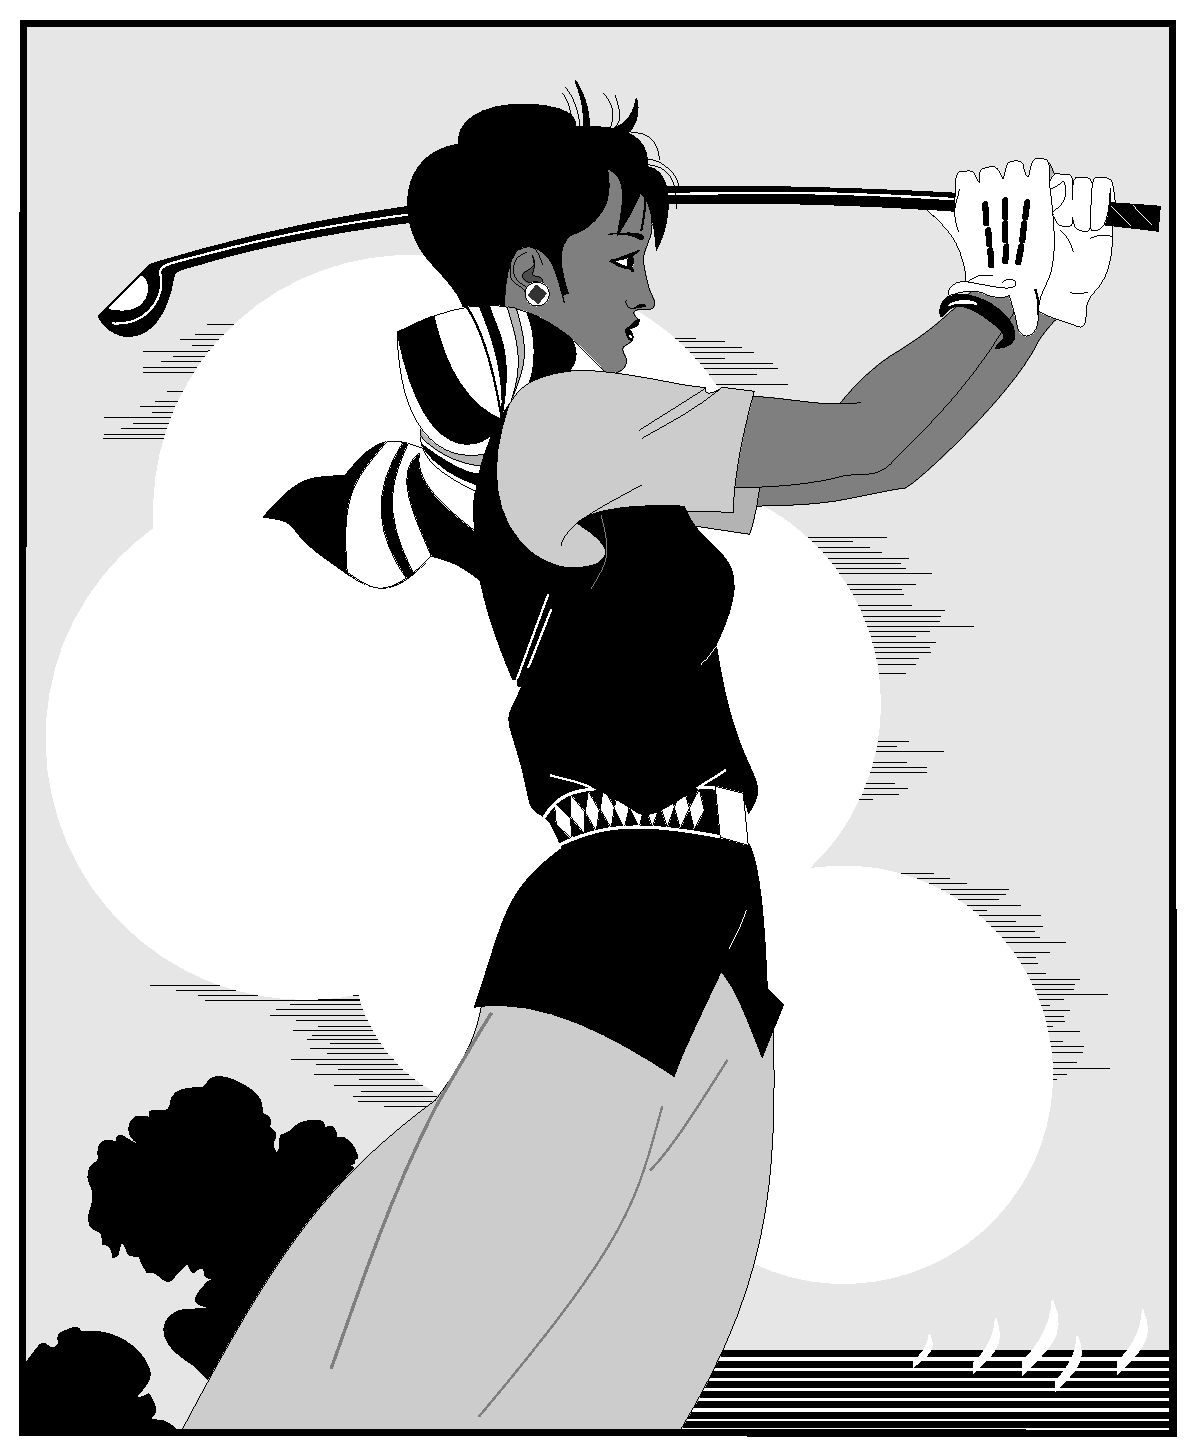
\includegraphics[width=0.4\textwidth]{golfer}}
\subfigure[打高尔夫球的人]{\label{golfer42}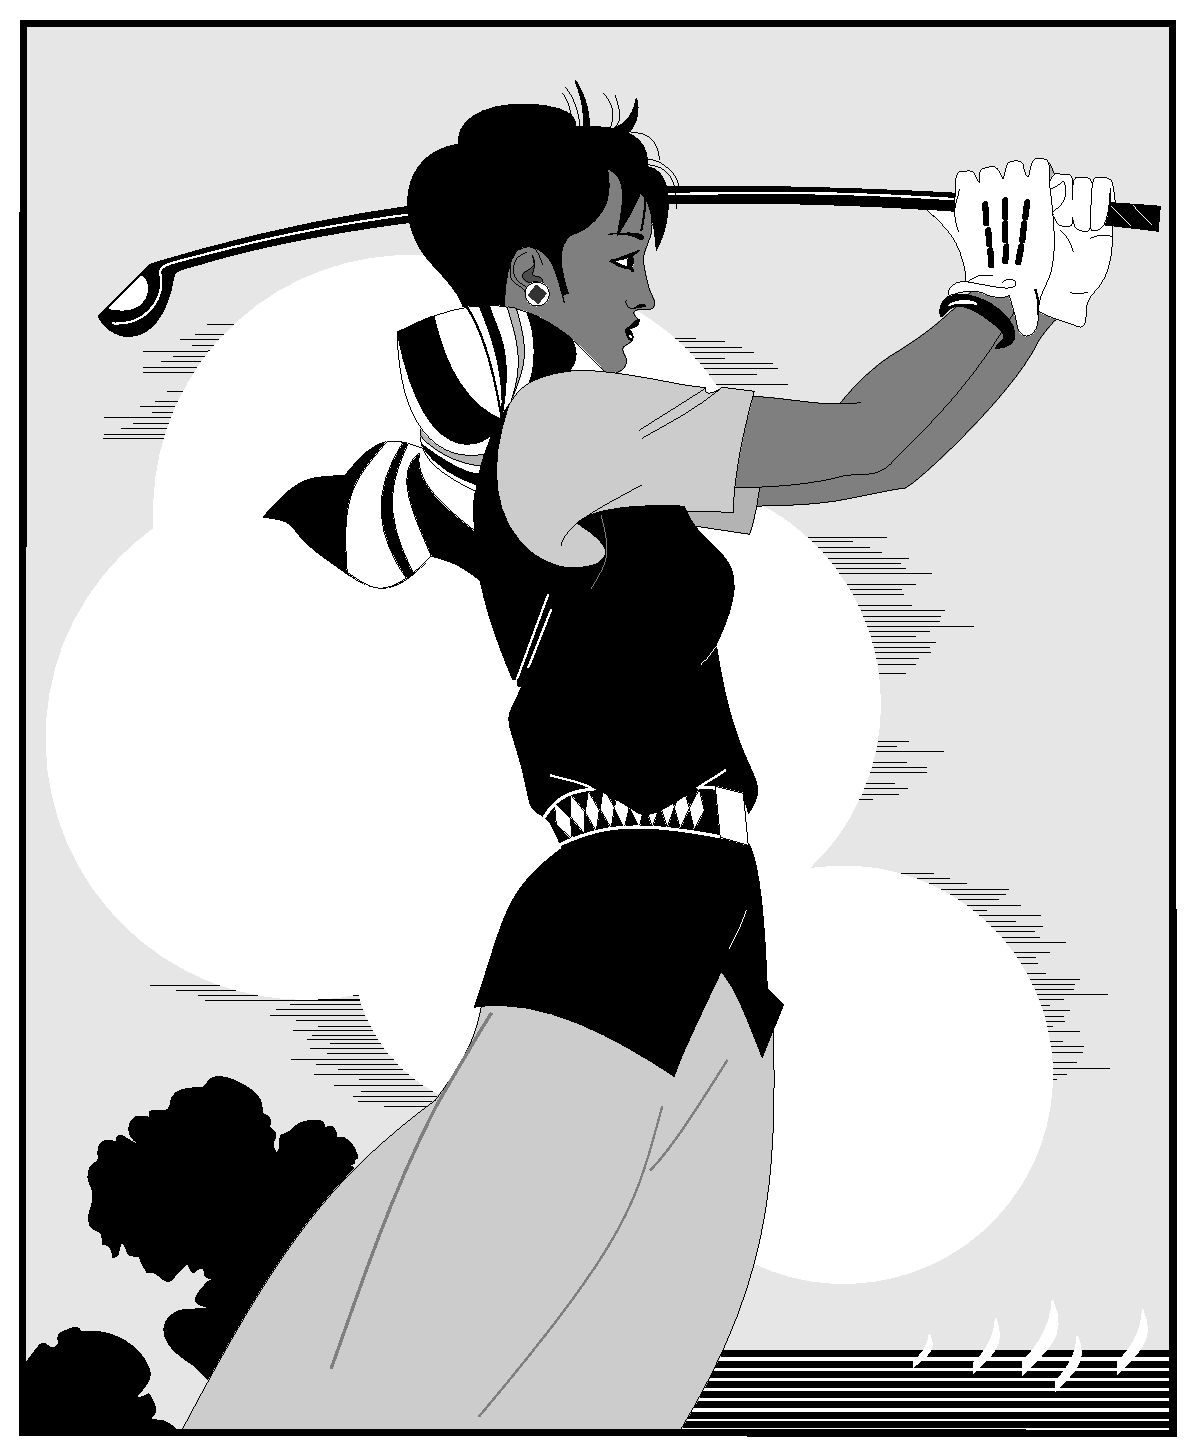
\includegraphics[width=0.4\textwidth]{golfer}}
\caption{打高尔夫球的人}\label{golfer4}\vspace{-1em}
\end{figure}

其代码及其说明如下。
\vspace{1em}\noindent\hrule
\begin{verbatim}
\begin{figure}[htbp]
\centering
\subfigure[第1个子图标题]{\label{第1个子图标签名}
                          \includegraphics[width=0.4\textwidth]{文件名}}
\subfigure[第2个子图标题]{\label{第2个子图标签名}
                          \includegraphics[width=0.4\textwidth]{文件名}}
\caption{中文总标题}\label{总标签名}
\vspace{-1em}
\end{figure}
\end{verbatim}
\noindent\hrule
\begin{verbatim}
引用方法:总图的引用方法同本章第1节,子图的引用方法用\ref{第n个子图标签名}来代替。
\end{verbatim}
\noindent\hrule\vspace{1em}

子图的引用示例:如图~\ref{golfer41}~和图~\ref{golfer42}~所示。

若想获得插图方法的更多信息,请参见网络上的~
Using Imported Graphics in \LaTeX and pdf\LaTeX~文档~http://tug.ctan.org/cgi-bin/ctanPackageInformation.py?id=epslatex。 
% !Mode:: "TeX:UTF-8" 

\section{表格的绘制方法}
\subsection{研究生院的绘表规范}

表应有自明性。表格不加左、右边线。表的编排建议采用国际通行的三线表。表中文字用宋体~5~号字。

每个表格均应有表题(由表序和表名组成)。表序一般按章编排,如第~1~章第一个插表的序号为“表~1-1”等。表序与表名之间空一格,
表名中不允许使用标点符号,表名后不加标点。表题置于表上,硕士学位论文只用中文,博士学位论文用中、英文两种文字居中排写,
中文在上,要求中文用宋体~5~号字,英文用新罗马字体~5~号字。

表头设计应简单明了,尽量不用斜线。表头中可采用化学符号或物理量符号。

全表如用同一单位,则将单位符号移至表头右上角,加圆括号。

表中数据应准确无误,书写清楚。数字空缺的格内加横线“-”(占~2~个数字宽度)。表内文字或数字上、下或左、右相同时,
采用通栏处理方式,不允许用“〃”、“同上”之类的写法。

表内文字说明,起行空一格、转行顶格、句末不加标点。

如某个表需要转页接排,在随后的各页上应重复表的编号。编号后加“(续表)”,表题可省略。续表应重复表头。

\subsection{普通表格的绘制方法}

表格应具有三线表格式,因此需要调用~booktabs~宏包,其标准格式如表~\ref{table1}~所示。
\begin{table}[htbp]
\caption{符合研究生院绘图规范的表格}
\vspace{-0.5em}\label{table1}\centering\zihao{5}
\begin{tabular}{ccccc}
\toprule
$D$(in) & $P_u$(lbs) & $u_u$(in) & $\beta$ & $G_f$(psi.in)\\
\midrule
 5 & 269.8 & 0.000674 & 1.79 & 0.04089\\
10 & 421.0 & 0.001035 & 3.59 & 0.04089\\
20 & 640.2 & 0.001565 & 7.18 & 0.04089\\
\bottomrule
\end{tabular}
\end{table}

其绘制表格的代码及其说明如下。
\vspace{1em}\noindent\hrule
\begin{lstlisting}
\begin{table}[htbp]
\caption{表格标题}
\vspace{-0.5em}\label{标签名}\centering\zihao{5}
\begin{tabular}{cc...c}
\toprule
表头第1个格   & 表头第2个格   & ... & 表头第n个格  \\
\midrule
表中数据(1,1) & 表中数据(1,2) & ... & 表中数据(1,n)\\
表中数据(2,1) & 表中数据(2,2) & ... & 表中数据(2,n)\\
...................................................\\
表中数据(m,1) & 表中数据(m,2) & ... & 表中数据(m,n)\\
\bottomrule
\end{tabular}
\end{table}
\end{lstlisting}
\noindent\hrule
\begin{lstlisting}
table环境是一个将表格嵌入文本的浮动环境。
\zihao{5}命令将表格的字号设置为五号字(10.5pt),在绘制表格结束退出时,不需要将字号再改回为\zihao{-4},正文字号默认为小四号字(12pt)。
tabular环境的必选参数由每列对应一个格式字符所组成:c表示居中,l表示左对齐,r表示右对齐,其总个数应与表的列数相同。此外,@{文本}可以出现在任意两个上述的列格式之间,其中的文本将被插入每一行的同一位置。表格的各行以\\分隔,同一行的各列则以&分隔。
\toprule、\midrule和\bottomrule三个命令是由booktabs宏包提供的,其中
\toprule和\bottomrule分别用来绘制表格的第一条(表格最顶部)和第三条(表格最底部)水平线,\midrule用来绘制第二条(表头之下)水平线,且第一条和第三条水平线的线宽大于第二条水平线的线宽。
引用方法:“如表~\ref{标签名}~所示”。
\end{lstlisting}
\noindent\hrule

\subsection{长表格的绘制方法}

长表格是当表格在当前页排不下而需要转页接排的情况下所采用的一种表格环境。若长表格仍按照普通表格的绘制方法来获得,
其所使用的\verb|table|浮动环境无法实现表格的换页接排功能,表格下方过长部分会排在表格第1页的页脚以下。为了能够实现长表格的转页接排功能,
需要调用~longtable~宏包,由于长表格是跨页的文本内容,因此只需要单独的\verb|longtable|环境,所绘制的长表格的格式如表~\ref{table2}~所示。

此长表格~\ref{table2}~第~2~页的标题“编号(续表)”和表头是通过代码自动添加上去的,无需人工添加,若表格在页面中的竖直位置发生了变化,长表格在第~2~页
及之后各页的标题和表头位置能够始终处于各页的最顶部,也无需人工调整,\LaTeX~系统的这一优点是~word~等软件所无法比拟的。

\zihao{5}\begin{longtable}{ccc}
\caption{中国省级行政单位一览\label{table2}}\vspace{-0.5em}\\
\toprule 名称 & 简称 & 省会或首府  \\ \midrule
\endfirsthead
\multicolumn{3}{c}{表~\thetable(续表)}\vspace{0.5em}\\
\toprule 名称 & 简称 & 省会或首府  \\ \midrule
\endhead
\bottomrule
\endfoot
北京市 & 京 & 北京\\
天津市 & 津 & 天津\\
河北省 & 冀 & 石家庄市\\
山西省 & 晋 & 太原市\\
内蒙古自治区 & 蒙 & 呼和浩特市\\
辽宁省 & 辽 & 沈阳市\\
吉林省 & 吉 & 长春市\\
黑龙江省 & 黑 & 哈尔滨市\\
黑龙江省 & 黑 & 哈尔滨市\\
黑龙江省 & 黑 & 哈尔滨市\\
黑龙江省 & 黑 & 哈尔滨市\\
黑龙江省 & 黑 & 哈尔滨市\\
黑龙江省 & 黑 & 哈尔滨市\\
上海市 & 沪/申 & 上海\\
江苏省 & 苏 & 南京市\\
浙江省 & 浙 & 杭州市\\
安徽省 & 皖 & 合肥市\\
福建省 & 闽 & 福州市\\
江西省 & 赣 & 南昌市\\
山东省 & 鲁 & 济南市\\
河南省 & 豫 & 郑州市\\
湖北省 & 鄂 & 武汉市\\
湖南省 & 湘 & 长沙市\\
广东省 & 粤 & 广州市\\
广西壮族自治区 & 桂 & 南宁市\\
海南省 & 琼 & 海口市\\
重庆市 & 渝 & 重庆\\
四川省 & 川/蜀 & 成都市\\
贵州省 & 黔/贵 & 贵阳市\\
云南省 & 云/滇 & 昆明市\\
西藏自治区 & 藏 & 拉萨市\\
陕西省 & 陕/秦 & 西安市\\
甘肃省 & 甘/陇 & 兰州市\\
青海省 & 青 & 西宁市\\
宁夏回族自治区 & 宁 & 银川市\\
新疆维吾尔自治区 & 新 & 乌鲁木齐市\\
香港特别行政区 & 港 & 香港\\
澳门特别行政区 & 澳 & 澳门\\
台湾省 & 台 & 台北市\\
\end{longtable}\zihao{-4}

绘制长表格的代码及其说明如下。
\vspace{1em}\noindent\hrule
\begin{lstlisting}

\zihao{5}\begin{longtable}{cc...c}
\caption{表格标题\label{标签名}}\vspace{-0.5em}\\
\toprule 表头第1个格 & 表头第2个格 & ... & 表头第n个格\\ \midrule
\endfirsthead
\multicolumn{n}{c}{表~\thetable(续表)}\vspace{0.5em}\\
\toprule 表头第1个格 & 表头第2个格 & ... & 表头第n个格\\ \midrule
\endhead
\bottomrule
\endfoot
表中数据(1,1) & 表中数据(1,2) & ... & 表中数据(1,n)\\
表中数据(2,1) & 表中数据(2,2) & ... & 表中数据(2,n)\\
...................................................\\
表中数据(m,1) & 表中数据(m,2) & ... & 表中数据(m,n)\\
\end{longtable}\zihao{-4}
\end{lstlisting}
\noindent\hrule
\begin{lstlisting}
在绘制长表格的前面留出一个空白行,并在第2行的一开始全局定义长表格的字号为五号字,这样能够保证长表格之前段落的行距保持不变。在绘制长表格结束后,需要\zihao{-4}命令重新将字号改为小四号字。
\endhead之前的文字描述的是第2页及其之后各页的标题或表头;\endfirsthead之前的文字描述的是第1页的标题和表头,若无此命令,则第1页的表头和标题由\endhead命令确定;同理,\endfoot之前的文字描述的是除最后一页之外每页的表格底部内容;\endlastfoot之前的文字描述的是最后一页的表格底部内容,若无此命令,则最后一页的表格底部内容由\endfoot命令确定;由于规范中长表格每页底部内容均相同(水平粗线),因此模板中没有用到\endlastfoot命令。
\end{lstlisting}
\noindent\hrule

\subsection{列宽可调表格的绘制方法}
论文中能用到列宽可调表格的情况共有两种,一种是当插入的表格某一单元格内容过长以至于一行放不下的情况,
另一种是当对公式中首次出现的物理量符号进行注释的情况,这两种情况都需要调用~tabularx~宏包。下面将分别对这两种情况下可调表格的绘制方法进行阐述。
\subsubsection{表格内某单元格内容过长的情况}

首先给出这种情况下的一个例子如表~\ref{table3}~所示。
\begin{table}[htbp]
\caption{最小的三个正整数的英文表示法}\label{table3}\vspace{-0.5em}\zihao{5}
\begin{tabularx}{\textwidth}{llX}
\toprule
Value & Name & Alternate names, and names for sets of the given size\\\midrule
1 & One & ace, single, singleton, unary, unit, unity\\
2 & Two & binary, brace, couple, couplet, distich, deuce, double, doubleton, duad, duality, duet, duo, dyad, pair, snake eyes, span, twain, twosome, yoke\\
3 & Three & deuce-ace, leash, set, tercet, ternary, ternion, terzetto, threesome, tierce, trey, triad, trine, trinity, trio, triplet, troika, hat-trick\\\bottomrule
\end{tabularx}
\end{table}

绘制这种表格的代码及其说明如下。
\vspace{1em}\noindent\hrule
\begin{lstlisting}
\begin{table}[htbp]
\caption{表格标题}\label{标签名}
\vspace{-0.5em}\zihao{5}
\begin{tabularx}{\textwidth}{l...X...l}
\toprule
表头第1个格   & ... & 表头第X个格   & ... & 表头第n个格  \\
\midrule
表中数据(1,1) & ... & 表中数据(1,X) & ... & 表中数据(1,n)\\
表中数据(2,1) & ... & 表中数据(2,X) & ... & 表中数据(2,n)\\
.........................................................\\
表中数据(m,1) & ... & 表中数据(m,X) & ... & 表中数据(m,n)\\
\bottomrule
\end{tabularx}
\end{table}
\end{lstlisting}
\noindent\hrule
\begin{lstlisting}
tabularx环境共有两个必选参数:第1个参数用来确定表格的总宽度,这里取为排版表格能达到的最大宽度——正文宽度\textwidth;第2个参数用来确定每列格式,其中标为X的项表示该列的宽度可调,其宽度值由表格总宽度确定。
标为X的列一般选为单元格内容过长而无法置于一行的列,这样使得该列内容能够根据表格总宽度自动分行。若列格式中存在不止一个X项,则这些标为X的列的列宽相同,因此,一般不将内容较短的列设为X。
标为X的列均为左对齐,因此其余列一般选为l(左对齐),这样可使得表格美观,但也可以选为c或r。
\end{lstlisting}
\noindent\hrule

\subsubsection{对物理量符号进行注释的情况}

为使得对公式中物理量符号注释的转行与破折号“\pozhehao ”后第一个字对齐,此处最好采用表格环境。此表格无任何线条,左对齐,
且在破折号处对齐,一共有“式中”二字、物理量符号和注释三列,表格的总宽度可选为文本宽度,因此应该采用\verb|tabularx|环境。
由\verb|tabularx|环境生成的对公式中物理量符号进行注释的公式如式(\ref{eq:1})所示。
\begin{equation}\label{eq:1}
\ddot{\bm{\rho}}-\frac{\mu}{R_t^3}\left(3\bm{R_t}\frac{\bm{R_t\rho}}{R_t^2}-\bm{\rho}\right)=\bm{a}
\end{equation}
\begin{tabularx}{\textwidth}{@{}l@{\quad}l@{\pozhehao }X@{}}
式中& $\bm{\rho}$ &追踪飞行器与目标飞行器之间的相对位置矢量;\\
&  $\ddot{\bm{\rho}}$&追踪飞行器与目标飞行器之间的相对加速度;\\
&  $\bm{a}$   &推力所产生的加速度;\\
&  $\bm{R_t}$ & 目标飞行器在惯性坐标系中的位置矢量;\\
&  $\omega_{t}$ & 目标飞行器的轨道角速度;\\
&  $\bm{g}$ & 重力加速度,$=\frac{\mu}{R_{t}^{3}}\left(
3\bm{R_{t}}\frac{\bm{R_{t}\rho}}{R_{t}^{2}}-\bm{\rho}\right)=\omega_{t}^{2}\frac{R_{t}}{p}\left(
3\bm{R_{t}}\frac{\bm{R_{t}\rho}}{R_{t}^{2}}-\bm{\rho}\right)$,这里~$p$~是目标飞行器的轨道半通径。
\end{tabularx}\vspace{\wordsep}

其中生成注释部分的代码及其说明如下。
\vspace{1em}\noindent\hrule
\begin{lstlisting}
\begin{tabularx}{\textwidth}{@{}l@{\quad}l@{\pozhehao}X@{}}
式中 & symbol-1 & symbol-1的注释内容;\\
     & symbol-2 & symbol-2的注释内容;\\
     .............................;\\
     & symbol-m & symbol-m的注释内容。
\end{tabularx}\vspace{\wordsep}
\end{lstlisting}
\noindent\hrule
\begin{lstlisting}
tabularx环境的第1个参数选为正文宽度,第2个参数里面各个符号的意义为:
    第1个@{}表示在“式中”二字左侧不插入任何文本,“式中”二字能够在正文中左对齐,若无此项,则“式中”二字左侧会留出一定的空白;
    @{\quad}表示在“式中”和物理量符号间插入一个空铅宽度的空白;
    @{\pozhehao}实现插入破折号的功能,\pozhehao是本模板定义的命令,其定义方式为
	\renewcommand{\pozhehao}{\raisebox{0.1em}{------}};
    第2个@{}表示在注释内容靠近正文右边界的地方能够实现右对齐。
\end{lstlisting}
\noindent\hrule\vspace{1em}
由此方法生成的注释内容应紧邻待注释公式并置于其下方,因此不能将代码放入\verb|table|浮动环境中。但此方法不能实现自动转页接排,
可能会在当前页剩余空间不够时,全部移动到下一页而导致当前页出现很大空白。因此在需要转页处理时,还请您手动将需要转页的代码放入一个
新的\verb|tabularx|环境中,将原来的一个\verb|tabularx|环境拆分为两个\verb|tabularx|环境。

若想获得绘制表格的更多信息,请参见网络上的~Tables in \LaTeXe: Packages and Methods~文档~http://www.tug.org/pracjourn/2007-1/mori/。 

% !Mode:: "TeX:UTF-8" 

\section{数学公式的输入方法}
\subsection{研究生院的公式规范}
论文中的公式应另起行,原则上应居中书写,与周围文字留有足够的空间区分开。
若公式前有文字(如“解”、“假定”等),文字空两格写,公式仍居中写。公式末不加标点。

公式应标注序号,并将序号置于括号内。 公式序号按章编排,如第~1~章第一个公式序号为“(1-1)”。公式的序号右端对齐。

公式较长时最好在等号“=”处转行,如难实现,则可在~$+$、$-$、$\times$、$\div$~运算符号处转行,转行时运算符号仅书写于转行式前,不重复书写。

文中引用公式时,一般用“见式~(1-1)”或“由公式~(1-1)”。

公式中用斜线表示“除”的关系时应采用括号,以免含糊不清,如~$a/(b\cos x)$。通常“乘”的关系在前,如~$a\cos x/b$而不写成~$(a/b)\cos x$。

不能用文字形式表示等式,如:$\textnormal{刚度}=\frac{{\textnormal{受力}}}{{\textnormal{受力方向的位移}}}$。




\textbf{对于数学公式的输入方法,网络上有一个比较全面权威的文档~Math mode~请大家事先大概浏览一下~http://tug.ctan.org/cgi-bin/ctanPackageInformation.py?id=voss-mathmode。下面将对学位论文中主要用到的数学公式排版形式进行阐述。}

\subsection{生成~\LaTeX~数学公式的两种方法}
对于先前没有接触过~\LaTeX~的人来说,编写~\LaTeX~数学公式是一件很繁琐的事,尤其是对复杂的数学公式来说,更可以说是一件难以完成的任务。
实际上,生成~\LaTeX~数学公式有两种较为简便的方法,一种是基于~MathType~数学公式编辑器的方法,另一种是基于~MATLAB~商业数学软件的方法,
下面将分别对这两种数学公式的生成方法作一下简单介绍。
\subsubsection{基于~MathType~软件的数学公式生成方法}
MathType~是一款功能强大的数学公式编辑器软件,能够用来在文本环境中插入~Windows OLE~图形格式的复杂数学公式,所以应用比较普遍。但此软件只有~30~天的试用期,之后若再继续使用则需要付费购买才行。网络上有很多破解版的~MathType~软件可供下载免费使用,
笔者推荐下载安装版本号在~6.5~之上的中文破解版。

在安装好~MathType~之后,若在输入窗口中编写数学公式,复制到剪贴板上的仍然是图形格式的对象。
若希望得到可插入到~\LaTeX~编辑器中的文本格式对象,则需要对~MathType~软件做一下简单的设置:在~MathType~最上排的按钮中依次选择“参数选项
$\to$转换”,在弹出的对话窗中选中“转换到其它语言(文字):”,在转换下拉框中选择“Tex~--~--~LaTeX 2.09 and later”,并将对话框最下方的两个复选框全部勾掉,点击确定,这样,再从输入窗口中复制出来的对象就是文本格式的了,就可以直接将其粘贴到~\LaTeX~
编辑器中了。按照这种方法生成的数学公式两端分别有标记\verb|\[|和标记\verb|\]|,在这两个标记之间才是真正的数学公式代码。

若希望从~MathType~输入窗口中复制出来的对象为图形格式,则只需再选中“公示对象(Windows OLE~图形)”即可。

\subsubsection{基于~MATLAB~软件的数学公式生成方法}
MATLAB~是矩阵实验室(Matrix Laboratory)的简称,是美国~MathWorks~公司出品的商业数学软件。它是当今科研领域最常用的应用软件之一,
具有强大的矩阵计算、符号运算和数据可视化功能,是一种简单易用、可扩展的系统开发环境和平台。

MATLAB~中提供了一个~latex~函数,它可将符号表达式转化为~\LaTeX~数学公式的形式。其语法形式为~latex(s),其中,~s~为符号表达式,
之后再将~latex~函数的运算结果直接粘贴到~\LaTeX~编辑器中。从~\LaTeX~数学公式中可以发现,其中可能包含如下符号组合:
\begin{verbatim*}
\qquad=两个空铅(quad)宽度
\quad=一个空铅宽度
\;=5/18空铅宽度
\:=4/18空铅宽度
\,=3/18空铅宽度
\!=-3/18空铅宽度
\ =一个空格
\end{verbatim*}
所以最好将上述符号组合从数学公式中删除,从而使数学公式显得匀称美观。

对于~word~等软件的使用者来说,在我们通过~MATLAB~运算得到符号表达式形式的运算结果时,在~word~中插入运算结果需要借助于~MathType~软件,
通过在~MathType~中输入和~MATLAB~运算结果相对应的数学表达形式,之后再将~MathType~数学表达式转换为图形格式粘贴到~word~中。实际上,
也可以将~MATLAB~中采用~latex~函数运行的结果直接粘贴到~MathType~中,再继续上述步骤,这样可以大大节省输入公式所需要的时间。
此方法在~MathType~6.5c~上验证通过,若您粘入到~MathType~中的仍然为从~MATLAB~中导入的代码,请您更新~MathType~软件。

\subsection{数学字体}
在数学模式下,常用的数学字体命令有如下几种:
\begin{verbatim}
\mathnormal或无命令 用数学字体打印文本;
\mathit             用斜体(\itshape)打印文本;
\mathbf             用粗体(\bfseries)打印文本;
\mathrm             用罗马体(\rmfamily)打印文本;
\mathsf             用无衬线字体(\sffamily)打印文本;
\mathtt             用打印机字体(\ttfamily)打印文本;
\mathcal            用书写体打印文本;
\end{verbatim}
在学位论文撰写中,只需要用到上面提到的~\verb|\mathit|、\verb|\mathbf|~和~\verb|\mathrm|~命令。若要得到~Times New Roman~的数学字体,则需要调用~txfonts~宏包(此宏包实际上采用的是~Nimbus Roman No9 L~字体,
它是开源系统中使用的免费字体,其字符字体与~Times New Roman~字体几乎完全相同);若要得到粗体数学字体,则需要调用~bm~宏包。表~\ref{table:fonts}~中分别列出了得到阿拉伯数字、拉丁字母和希腊字母
各种数学字体的命令。
\begin{table}[htbp]
\caption{常用数学字体命令一览}
\vspace{-0.5em}\label{table:fonts}\centering\zihao{5}
\begin{tabular}{llll}
\toprule
 & 阿拉伯数字\&大写希腊字母 & 大小写拉丁字母 & 小写希腊字母  \\
\midrule
斜体 & \verb|\mathit{}| & \verb|无命令| & \verb|无命令|\\
粗斜体 & \verb|\bm{\mathit{}}| & \verb|\bm{}| & \verb|\bm{}|\\
直立体 & \verb|无命令| & \verb|\mathrm{}| & \verb|字母后加up|\\
粗体 & \verb|\mathbf{}或\bm{}| & \verb|\mathbf{}| & \verb|\bm{字母后加up}|\\
\bottomrule
\end{tabular}
\end{table}

\noindent 下面列出了一些应采用直立数学字体的数学常数和数学符号。

\vspace{-0.5em}\begin{center}\begin{tabularx}{0.7\textwidth}{XX}
$\mathrm{d}$、 $\mathrm{D}$、 $\mathrm{p}$~\pozhehao 微分算子 & $\mathrm{e}$~\pozhehao 自然对数之底数\\
$\mathrm{i}$、 $\mathrm{j}$~\pozhehao 虚数单位 & $\piup$\pozhehao 圆周率\\
\end{tabularx}\end{center}

\subsection{行内公式}
出现在正文一行之内的公式称为行内公式,例如~$f(x)=\int_{a}^{b}\frac{\sin{x}}{x}\mathrm{d}x$。对于非矩阵和非多行形式的行内公式,
一般不会使得行距发生变化,而~word~等软件却会根据行内公式的竖直距离而自动调节行距,如图~\ref{hangju}~所示。

\begin{figure}[htbp]
\centering
\subfigure[由~\LaTeX~系统生成的行内公式]{\label{latex}{\fbox{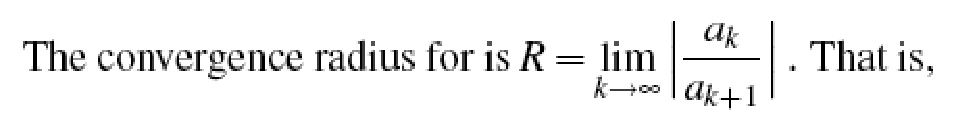
\includegraphics[width=0.55\textwidth]{latex}}}}
\subfigure[由~word软件生成的~.doc~格式行内公式]{\label{word}\fbox{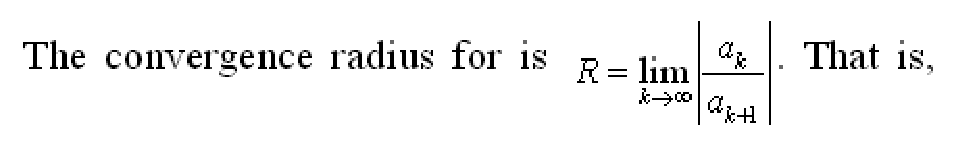
\includegraphics[width=0.55\textwidth]{word}}}
\subfigure[由~word软件生成的~.pdf~格式行内公式]{\label{pdf}\fbox{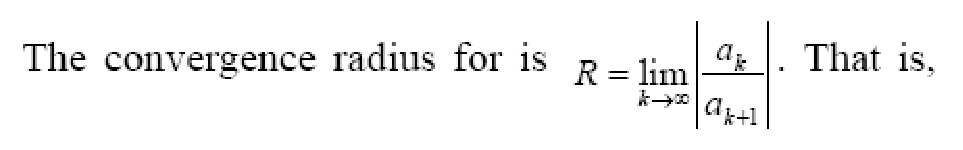
\includegraphics[width=0.55\textwidth]{pdf}}}
\caption{由~\LaTeX~和~word~生成的~3~种行内公式屏显效果}\label{hangju}
\vspace{-1em}
\end{figure}
这三幅图分别为~\LaTeX~和~word~生成的行内公式屏显效果,从图中可看出,在~\LaTeX~文本含有公式的行内,在正文与公式之间对接工整,行距不变;而在~word~文本含有公式的行内,在正文与公式之间对接不齐,行距变大。因此从这一点来说,
\LaTeX~系统在数学公式的排版上具有很大优势。

\LaTeX~提供的行内公式最简单、最有效的方法是采用~\TeX~本来的标记\pozhehao 开始和结束标记都写作~\$,例如本段开始的例子可由下面的输入得到。

\verb|$f(x)=\int_{a}^{b}\frac{\sin{x}}{x}\mathrm{d}x$|

\subsection{行间公式}
位于两行之间的公式称为行间公式,每个公式都是一个单独的段落,例如
\[\int_a^b{f\left(x\right)\mathrm{d}x}=\lim_{\left\|\Delta{x_i}\right\|\to 0}\sum_i{f\left(\xi_i\right)\Delta{x_i}}\]
除人工编号外,\LaTeX~各种类型行间公式的标记见表~\ref{eqtag}。
\begin{table}[htbp]
\caption{各种类型行间公式的标记}\label{eqtag}
\vspace{-0.5em}\centering\zihao{5}
\begin{tabularx}{0.85\textwidth}{cXX}
\toprule
& 无编号 & 自动编号\\\midrule
单行公式 & \verb|\begin{displaymath}...... \end{displaymath}|~或~\verb|\[...\]| & \verb|\begin{equation} ...... \end{equation}|\\
多行公式 & \verb|\begin{eqnarray*} ...... \end{eqnarray*}| & \verb|\begin{eqnarray} ...... \end{eqnarray}|\\
\bottomrule
\end{tabularx}
\end{table}
另外,在自动编号的某行公式行尾添加标签~\verb|\nonumber|,可将该行转换为无编号形式。

行间多行公式需采用~\verb|eqnarray|~或~\verb|eqnarray*|~环境,它默认是一个列格式为~\verb|rcl|~的~3~列矩阵,并且中间列的字号要小一些,因此通常只将需要对齐的运算符号(通常为等号“=”)置于中间列。

\subsection{可自动调整大小的定界符}
若在左右两个定界符之前分别添加命令~\verb|\left|~和~\verb|\right|,则定界符可根据所包围公式大小自动调整其尺寸,这可从式(\ref{nodelimiter})和式(\ref{delimiter})中看出。
\begin{equation}\label{nodelimiter}
(\sum_{k=\frac12}^{N^2})
\end{equation}
\begin{equation}\label{delimiter}
\left(\sum_{k=\frac12}^{N^2}\right)
\end{equation}
式(\ref{nodelimiter})和式(\ref{delimiter})是在~\LaTeX~中分别输入如下代码得到的。
\begin{verbatim}
(\sum_{k=\frac12}^{N^2})
\left(\sum_{k=\frac12}^{N^2}\right)
\end{verbatim}
\verb|\left|~和~\verb|\right|~总是成对出现的,若只需在公式一侧有可自动调整大小的定界符,则只要用“.”代替另一侧那个无需打印出来的定界符即可。

若想获得关于此部分内容的更多信息,可参见~Math mode~文档的第~8~章“Brackets, braces and parentheses”。

\subsection{数学重音符号}
数学重音符号通常用来区分同一字母表示的不同变量,输入方法如下(需要调用~\verb|amsmath|~宏包):

\vspace{0.5em}\noindent\zihao{5}\begin{tabularx}{\textwidth}{Xc|Xc|Xc}
 \verb|\acute| & $\acute{a}$ & \verb|\mathring| & $\mathring{a}$ & \verb|\underbrace| & $\underbrace{a}$ \\
 \verb|\bar| & $\bar{a}$ & \verb|\overbrace| & $\overbrace{a}$ & \verb|\underleftarrow| & $\underleftarrow{a}$ \\
 \verb|\breve| & $\breve{a}$ & \verb|\overleftarrow| & $\overleftarrow{a}$ & \verb|\underleftrightarrow| & $\underleftrightarrow{a}$ \\
 \verb|\check| & $\check{a}$ & \verb|\overleftrightarrow| & $\overleftrightarrow{a}$ & \verb|\underline| & $\underline{a}$ \\
 \verb|\dddot| & $\dddot{a}$ & \verb|\overline| & $\overline{a}$ & \verb|\underrightarrow| & $\underrightarrow{a}$ \\
 \verb|\ddot| & $\ddot{a}$ & \verb|\overrightarrow| & $\overrightarrow{a}$ & \verb|\vec| & $\vec{a}$ \\
 \verb|\dot| & $\dot{a}$ & \verb|\tilde| & $\tilde{a}$ & \verb|\widehat| & $\widehat{a}$ \\
 \verb|\grave| & $\grave{a}$ & \verb|\underbar| & $\underbar{a}$ & \verb|\widetilde| & $\widetilde{a}$ \\
 \verb|\hat| & $\hat{a}$ 
\end{tabularx}\vspace{0.5em}
\zihao{-4} 当需要在字母~$i$~和~$j$~的上方添加重音符号时,为了去掉这两个字母顶上的小点,这两个字母应该分别改用~\verb|\imath|~和~\verb|\jmath|。

如果遇到某些符号不知道该采用什么命令能输出它时,则可通过

http://detexify.kirelabs.org/classify.html~\pozhehao Detexify$^2$~网站来获取符号命令。若用鼠标左键在此网页的方框区域内画出你所要找的符号形状,则会在网页右方列出和你所画符号形状相近的~5~个符号及其相对应的~\LaTeX~输入命令。若所列出的符号中不包括你所要找的符号,还可通过点击“Select from the complete list!”的链接以得分从低到高的顺序列出所有符号及其相对应的~\LaTeX~输入命令。

最后,笔者建议大家还是要以~Math mode~这篇~pdf~文档作为主要参考。若要获得最为标准、美观的数学公式排版形式,可以查查文档中是否有和你所要的排版形式相同或相近的代码段,通过修改代码段以获得你所要的数学公式排版形式。
% !Mode:: "TeX:UTF-8" 

\section{模板的其它说明}

\subsection{单层罗列环境}
哈工大学位论文一般可采用两种罗列环境:一种是并列条目有同样标签的~\verb|itemize|~罗列环境,另一种是具有自动排序编号符号的~\verb|enumerate|~罗列环境。这两种罗列环境的样式参数可参考图~\ref{list}。
\begin{figure}[htbp]
\centering
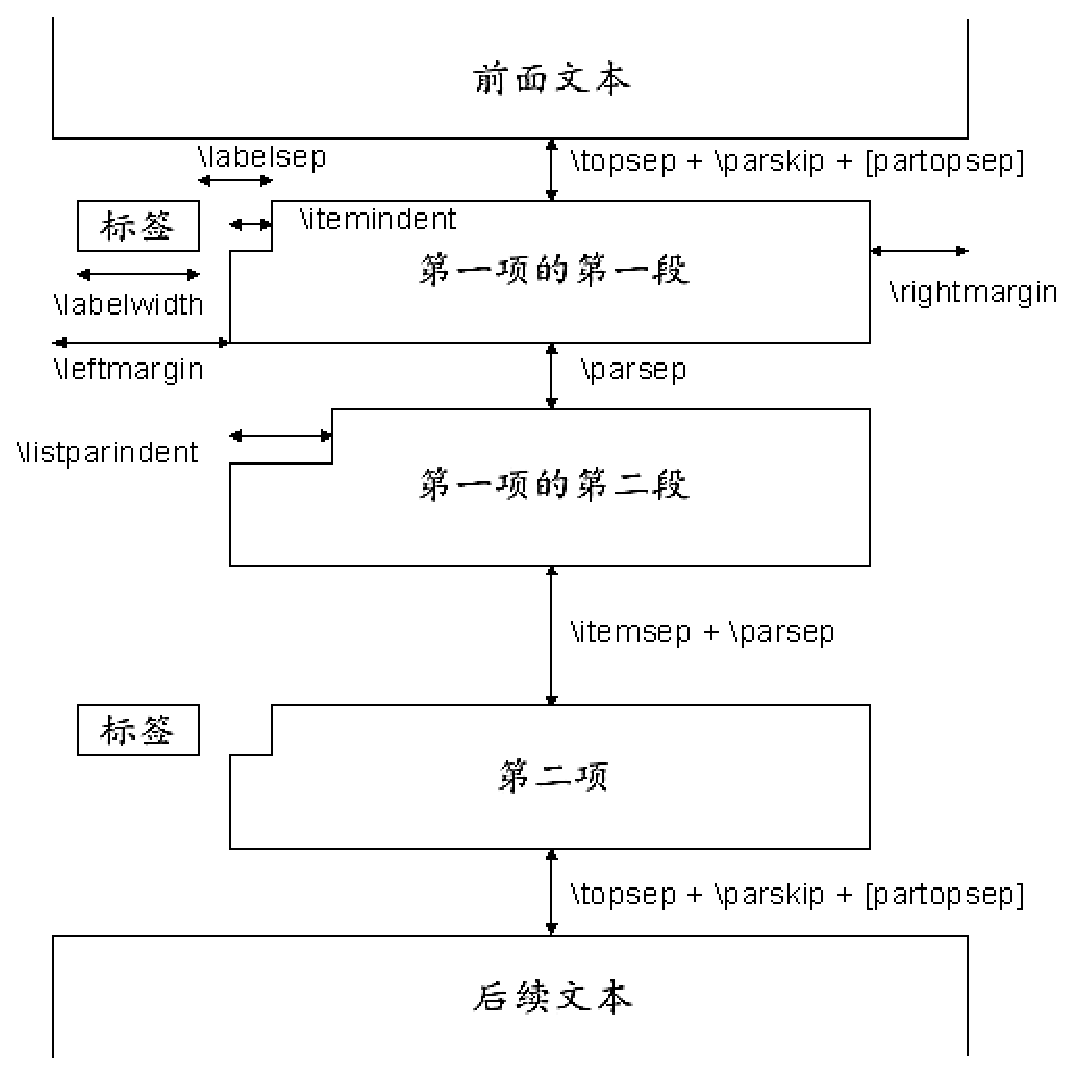
\includegraphics[width = 0.6\textwidth]{list}
\caption{罗列环境参数示意图}\label{list}\vspace{-1em}
\end{figure}
通过调用~enumitem~宏包可以很方便地控制罗列环境的布局,其~format.tex~文件中的~\verb|\setitemize|~和~\verb|\setenumerate|~命令分别用来设置~\verb|itemize|~和~\verb|enumerate|~环境的样式参数。采用~\verb|itemize|~单层罗列环境的排版形式如下:
\begin{itemize}
\item 第一个条目文本内容
\item 第二个条目文本内容
\item 第三个条目文本内容
\end{itemize}
其代码如下
\begin{verbatim}
\begin{itemize}
  \item 第一个条目文本内容
  \item 第二个条目文本内容
  ...
  \item 第三个条目文本内容
\end{itemize}
\end{verbatim}
采用~\verb|enumerate|~单层罗列环境的排版形式如下:
\begin{enumerate}
\item 第一个条目文本内容
\item 第二个条目文本内容
\item 第三个条目文本内容
\end{enumerate}
其代码如下
\begin{verbatim}
\begin{enumerate}
  \item 第一个条目文本内容
  \item 第二个条目文本内容
  ...
  \item 第三个条目文本内容
\end{enumerate}
\end{verbatim}

\subsection{定理定义}

若需要书写定理定义等内容,而且带有顺序编号,需要采用如下环境。除了~\verb|proof|~环境之外,其余~9~个环境都可以有一个可选参数作为附加标题。

\begin{center}\vspace{0.5em}\noindent\zihao{5}\begin{tabularx}{0.7\textwidth}{lX|lX}
定理 & \verb|theorem|~环境 & 定义 & \verb|definition|~环境 \\
例 & \verb|example|~环境 & 算法 & \verb|algo|~环境 \\
公理 & \verb|axiom|~环境 & 命题 & \verb|proposition|~环境 \\
引理 & \verb|lemma|~环境 & 推论 & \verb|corollary|~环境 \\
注解 & \verb|remark|~环境 & 证明 & \verb|proof|~环境 \\
\end{tabularx}\end{center}


\bibliographystyle{GBT7714-2005NLang-HIT}
\addtolength{\bibsep}{-0.8em}
\nocite{*}
\bibliography{reference}

\end{document}
